\documentclass[11pt,a4paper]{article}

% ---------- Packages ----------
\usepackage[utf8]{inputenc}
\usepackage[T1]{fontenc}
\usepackage{lmodern}
\usepackage{amsmath,amssymb}
\usepackage{enumitem}
\usepackage{geometry}
\usepackage{fancyhdr}
\usepackage[most]{tcolorbox}   % enhanced, breakable
\usepackage{hyperref}

% ---------- Geometry ----------
\geometry{margin=2.5cm}

% ---------- Header/Footer ----------
\setlength{\headheight}{14pt}  % fancyhdr warning verhindern
\pagestyle{fancy}
\fancyhf{}
\lhead{Einführung in die Elektrotechnik}
\rhead{Wintersemester 2025}
\cfoot{\thepage}

% ---------- Exercise Environment ----------
\newcounter{exercise}
\newenvironment{exercise}[1][]
  {\refstepcounter{exercise}%
   \begin{tcolorbox}[enhanced, breakable, width=\textwidth,
     colback=blue!5!white,colframe=blue!60!black,
     fonttitle=\bfseries\large,
     title=Aufgabe~\theexercise:~#1]}
  {\end{tcolorbox}}

% ---------- Solution Environment ----------
\newif\ifshowsolutions
\showsolutionstrue  % comment to hide solutions

\newenvironment{solution}
  {\ifshowsolutions
     \begin{tcolorbox}[enhanced, breakable, width=\textwidth,
       colback=green!5!white,colframe=green!50!black,
       fonttitle=\bfseries\large,
       title=Lösung]}
  {\end{tcolorbox}\fi}

% ---------- Document ----------
\begin{document}

% ----- Header Box -----
\begin{tcolorbox}[enhanced, breakable, colback=gray!10!white,
  colframe=gray!70!black, fonttitle=\bfseries\large,
  title={Aufgabenblatt \#4}: Magnetisches Feld, sharp corners, width=\textwidth]
\begin{center}
  Besprechung: 17.11.2025
\end{center}
\end{tcolorbox}
\vspace{1cm}

% ----- Exercise 1 -----
\begin{exercise}[Magnetische Kraft]
In einem geraden, stromführenden Abschnitt eines Leiters befindet sich ein Stromelement
\[
I \vec{l}
\]
mit
\[
I = 2.7~\text{A}, \quad \vec{l} = (3.0\,\hat{x} + 4.0\,\hat{y})~\text{cm}.
\]
Es ist umgeben von einem homogenen Magnetfeld
\[
\vec{B} = 1.3\,\hat{x}~\text{T}.
\]
Berechne die auf den Leiterabschnitt wirkende Kraft.
\end{exercise}

\ifshowsolutions
\begin{solution}
Magnetische Kraft:
\[
\vec{F} = I (\vec{l} \times \vec{B})
\]

Berechnung des Kreuzprodukts:
\[
\begin{aligned}
(\vec{l} \times \vec{B})_x &= l_y B_z - l_z B_y = 0.04 \cdot 0 - 0 \cdot 0 = 0,\\[4pt]
(\vec{l} \times \vec{B})_y &= l_z B_x - l_x B_z = 0 \cdot 1.3 - 0.03 \cdot 0 = 0,\\[4pt]
(\vec{l} \times \vec{B})_z &= l_x B_y - l_y B_x = 0.03 \cdot 0 - 0.04 \cdot 1.3 = -0.052.
\end{aligned}
\]

\[
\Rightarrow \quad \vec{l} \times \vec{B} = -0.052\,\hat{z}~\text{m·T}
\]

Demnach:
\[
\vec{F} = 2.7~\text{A} \cdot (-0.052)\,\hat{z}~\text{m·T} = -0.14\,\hat{z}~\text{N}
\]
\end{solution}
\fi

% ----- Exercise 2 -----
\begin{exercise}[Lorentz-Kraft]
Ein Geschwindigkeitsfilter arbeitet mit einem Magnetfeld von \( B = 0.28\,\text{T} \), das senkrecht zu einem elektrischen Feld von \( E = 0.46\,\text{MV/m} \) steht. Wie schnell muss sich ein Teilchen bewegen, um den Filter ohne Ablenkung zu durchlaufen?
\end{exercise}

\ifshowsolutions
\begin{solution}
Elektrische und die magnetische Kraft müssen sich gegenseitig ausgleichen:
\[
qE = qvB
\]

\[
\Rightarrow v = \frac{E}{B} = \frac{0.46 \times 10^{6}\,\text{V/m}}{0.28\,\text{T}} = 1.64 \times 10^{6}\,\text{m/s}
\]
\end{solution}
\fi

% ----- Exercise 3 -----
\begin{exercise}[Ampèresches Gesetz]
Durch einen langen, geraden, dünnwandigen, Hohlzylinder mit Radius $r$ fließt ein Strom $I$ parallel zu seiner Längsachse. Wie lauten Betrag und Richtung der Magnetfelder innerhalb und außerhalb des Hohlzylinders?
\end{exercise}

\ifshowsolutions
\begin{solution}
Innerhalb des Hohlzylinders ($r_{\text{inside}} < r$):

Da der Zylinder dünnwandig ist und der Strom nur an der Oberfläche fließt, ist nach dem Ampèreschen Gesetz das Magnetfeld innerhalb des Zylinders gleich null:
\[
\vec{B}_{\text{inside}} = 0
\]

\bigskip

Außerhalb des Hohlzylinders ($r_{\text{outside}} > r$):

Für Punkte außerhalb des Zylinders kann das Magnetfeld mit dem Ampèreschen Gesetz berechnet werden. Wählt man eine zum Zylinder konzentrische Schleife mit Radius $r_{\text{outside}}$, ergibt sich für den Betrag des Magnetfeldes:
\[
B_{\text{outside}} = \frac{\mu_0 I}{2 \pi r_{\text{outside}}},
\]
wobei $\mu_0$ die Permeabilität des Vakuums ist.

Die Richtung des Magnetfeldes folgt der Rechte-Hand-Regel: Wenn die Finger der rechten Hand den Zylinder in Stromrichtung umschließen, zeigt der Daumen entlang der Stromachse und das Magnetfeld verläuft tangential zur Schleife um den Zylinder.
\end{solution}
\fi

% ----- Exercise 4 -----
\begin{exercise}[Faradaysches Gesetz: Bewegter Leiter]
Eine rechteckige Leiterschleife hat die Breite $l=0.2\,\text{m}$ (die Seite, die die Feldgrenze durchquert) und die Höhe $h=0.1\,\text{m}$. Die Schleife liegt anfänglich vollständig in einem Bereich eines homogenen Magnetfeldes $B$, das in die Zeichenebene hinein (vom Betrachter weg) gerichtet ist, mit dem Betrag $B=0.8\,\text{T}$. Die Schleife wird mit konstanter Geschwindigkeit $v=0.5\,\frac{\text{m}}{\text{s}}$ nach rechts gezogen, sodass sie den Magnetfeldbereich verlässt.
\begin{enumerate}[label=\alph*)]
  \item Wie ist der Betrag der induzierten Spannung in der Schleife, während sie sich teilweise aus dem Magnetfeldbereich herausbewegt?
  \item Welche Richtung (im Uhrzeigersinn oder gegen den Uhrzeigersinn) hat der induzierte Strom aus Perspektive des Beobachters? Begründe dies mithilfe der Lenzschen Regel.
\end{enumerate}
\end{exercise}

\ifshowsolutions
\begin{solution}
Der magnetische Fluss durch den Teil der Leiterschleife innerhalb des Magnetfeldes ist $\Phi=B\,A_{\rm in}$. Wenn die Schleife den Bereich verlässt, nimmt $A_{\rm in}$ ab, also ist $d\Phi/dt<0$. Das Faradaysche Gesetz ergibt
\[
V = -\frac{d\Phi}{dt}\,,
\]
und für die gerade Seite, die sich mit der Geschwindigkeit $v$ bewegt, beträgt der Betrag der induzierten Spannung
\[
|V| = B \cdot l \cdot v\,.
\]

\begin{enumerate}[label=\alph*)]
\item Betrag:
\[
|V| = B \cdot l \cdot v = 0.8\,\text{T} \cdot 0.2\,\text{m} \cdot 0.5\,\frac{\text{m}}{\text{s}} = 0.08\,\text{V}
\]

\item Richtung:
Der magnetische Fluss (in die Zeichenebene hinein) nimmt ab, während die Schleife den Bereich verlässt. Nach der Lenzschen Regel wird der induzierte Strom ein Magnetfeld erzeugen, das versucht den verlorenen Fluss aufrechtzuerhalten – das heißt ein in die Zeichenebene hinein zeigendes Magnetfeld. Die Leiterschleife kann als Mini Elektromagnet (Spule) angesehen werden. Verwendet man also die Rechte-Hand-Regel (Finger zeigen in Richtung des Stroms, der Daumen zeigt die Richtung des Magnetfeldes an), so entspricht ein Magnetfeld, das in die Zeichenebene hinein gerichtet ist, einem vom Beobachter aus gesehen im Uhrzeigersinn verlaufenden Strom. Daher ist der induzierte Strom im Uhrzeigersinn gerichtet.
\end{enumerate}
\end{solution}
\fi

% ----- Exercise 5 -----
\begin{exercise}[Faradaysches Gesetz: Veränderliches Feld]
Eine kreisförmige Leiterschleife mit Radius $r=5\,\text{cm}$ befindet sich in einem Bereich, in dem das senkrecht zur Schleife gerichtete Magnetfeld zeitlich zunimmt gemäß
\[
B(t) = 0.012\,t\,\text{T}\quad\text{mit }t\text{ in Sekunden.}
\]
Der Widerstand der Leiterschleife beträgt $R = 2\,\Omega$.  

\begin{enumerate}[label=\alph*)]
  \item Was ist der Betrag der induzierten Spannung bei $t=4\,\text{s}$?
  \item Was ist der Betrag des induzierten Stromes zu dieser Zeit? Und wie ist er gerichtet (im oder gegen den Uhrzeigersinn), falls $B$ aus der Zeichenebene heraus zeigt?
\end{enumerate}
\end{exercise}

\ifshowsolutions
\begin{solution}
Der magnetische Fluss durch die Leiterschleife beträgt $\Phi(t)=B(t) \cdot \pi r^{2}$. Damit ist der Betrag der induzierten Spannung gemäß dem Faradayschen Gesetz
\[
|V| = \left|\frac{d\Phi}{dt}\right| = \pi r^{2} \cdot \left|\frac{dB}{dt}\right|.
\]
$dB/dt$ ist konstant, da $B(t) = 0.012\,t\,\text{T}$.

\begin{enumerate}[label=\alph*)]
\item Betrag: Radius $r=0.05\,\text{m}$ und $dB/dt=0.012\ \mathrm{T/s}$. Somit gilt
\[
|V|=\pi \cdot 0.05^2 \cdot 0.012\,\mathrm{V} \approx 9.42\times10^{-5}\,\mathrm{V}.
\]

\item Induzierter Strom und Richtung: Gemäß Ohmschem Gesetz gilt
\[
I = |V|/R = \frac{9.42 \times 10^-5}{2}\,\mathrm{A} \approx 4.71 \times 10^{-5}\,\mathrm{A}.
\]
Richtung: Da $B$ aus der Zeichenebene heraus zunimmt, muss das induzierte Magnetfeld dieser Zunahme entgegenwirken und ist daher in die Zeichenebene hinein gerichtet. Ein in die Zeichenebene hinein zeigendes Magnetfeld entspricht einem im Uhrzeigersinn verlaufenden induzierten Strom (vom Beobachter aus gesehen).
\end{enumerate}
\end{solution}
\fi

% ----- Exercise 6 -----
\begin{exercise}[Zeitabhängige Spulenspannungen und -ströme]
Wie groß ist der Strom $i(t)$ für $0 < t < 2$ Sekunden, wenn die unten dargestellte Spannungsform an eine Induktivität von $10\text{-mH}$ angelegt wird? Es gilt die Anfangsbedingung $i(0) = 0$.

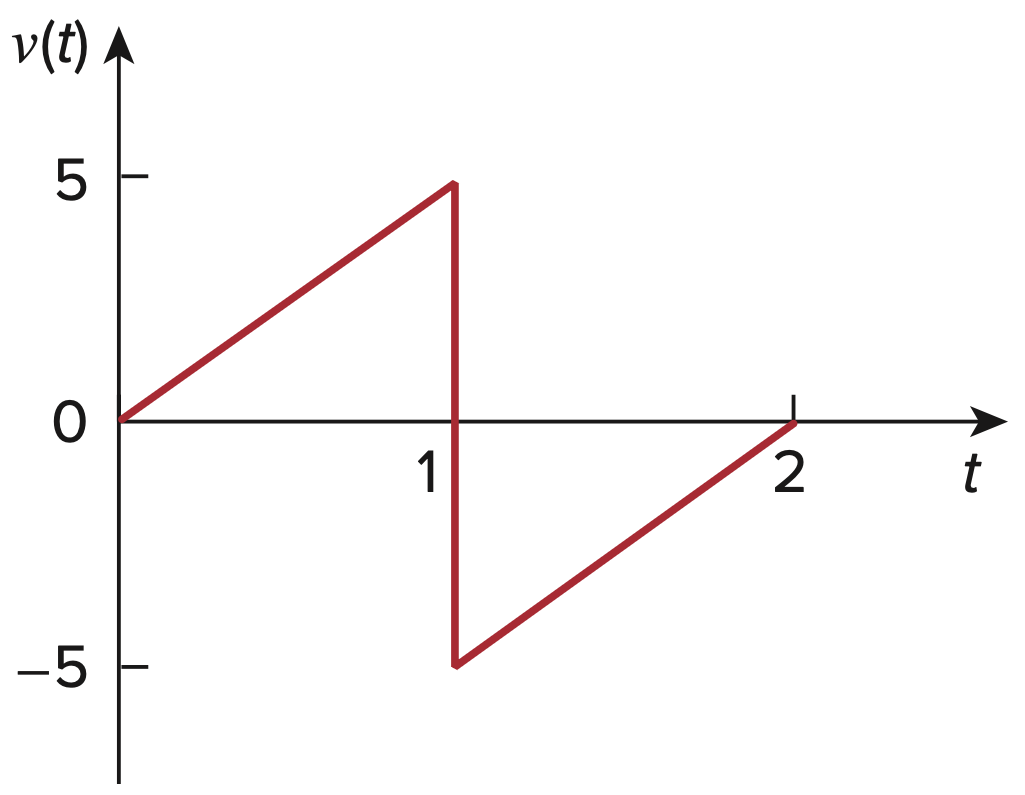
\includegraphics[width=0.5\textwidth]{figures/inductor_VI.png}
\end{exercise}

\ifshowsolutions
\begin{solution}
Für eine Induktivität gilt:
\[
v(t) = L \frac{di(t)}{dt}
\]

$0 < t < 1\,\text{s}$ (Zunahme $0$ → $5\,\text{V}$):

\[
v(t) = 5 t\,\mathrm{V} \quad \Rightarrow \quad \frac{di}{dt} = \frac{5 t\,\mathrm{V}}{0.01\,\mathrm{H}} = 500 t\,\mathrm{A/s}
\]

Integrieren ergibt:
\[
i(t) = \int 500 t\,\mathrm{A/s} \, dt = (250 t^2 + C)\,\mathrm{A}
\]

Da $i(0) = 0$, $C=0$:
\[
\boxed{i(t) = 250 t^2\,\mathrm{A}, \quad 0 < t < 1}
\]

\bigskip

$t = 1\,\text{s}$ (instantaner Abfall $5$ → $-5\,\text{V}$):

Eine ideale Induktivität kann den Strom nicht sprunghaft ändern. Daher ist der Strom bei $t=1$ stetig:
\[
i(1^-) = i(1^+) = 250\,\text{A}
\]

Der instantane Sprung in der Spannung entspricht einer endlichen Änderung der Steigung $di/dt$, $i(t)$ selbst ist stetig.

\bigskip

$1 < t < 2\,\text{s}$ (Zunahme $-5$ → $0\,\text{V}$):

Die Spannung ist jetzt
\[
v(t) = -5\,\text{V} + 5 (t-1)\,\text{V} = (5 t - 10)\,\text{V}, \quad 1 < t < 2.
\]

Daher gilt
\[
\frac{di}{dt} = \frac{(5 t - 10)\,\text{V}}{0.01,\mathrm{H}} = (500 t - 1000)\,\mathrm{A/s}.
\]

Integrieren ergibt:
\[
i(t) = \int (500 t - 1000)\,\mathrm{A/s} dt = (250 t^2 - 1000 t + C)\,\mathrm{A}
\]

Kontinuität bei $t = 1$: $i(1) = 250\,\mathrm{A}$
\[
250\,\mathrm{A} = (250(1)^2 - 1000(1) + C)\,\mathrm{A} \implies C = 1000
\]

Somit gilt:
\[
\boxed{i(t) = (250 t^2 - 1000 t + 1000)\,\mathrm{A}, \quad 1 < t < 2}
\]
\end{solution}
\fi

% ----- Exercise 7 -----
\begin{exercise}[Coil]
Durch eine Zylinderspule mit einer Länge von $2.7 \,\mathrm{m}$, einem Radius von $0.85 \,\mathrm{cm}$ und 600 Windungen fließt ein Strom von $2.5 \,\mathrm{A}$. Wie groß ist $B$ im Innern der Spule, weit entfernt von den Enden?
\end{exercise}

\ifshowsolutions
\begin{solution}
Das Magnetfeld im Innern eines langen Solenoiden (weit entfernt von den Enden) ist gegeben durch
\[
B = \mu_0 \, n \, I,
\]
wobei $n$ die Anzahl der Windungen pro Einheitslänge ist:
\[
n = \frac{N}{l} = \frac{600}{2.7 \,\mathrm{m}} \approx 222.22 \,\mathrm{turns/m}
\]

Mit der Vakuumpermeabilität
\[
\mu_0 = 4\pi \cdot 10^{-7} \,\mathrm{H/m}
\]
ergibt sich folgendes Magnetfeld:
\[
B = (4 \pi \cdot 10^{-7}) \cdot 222.22 \cdot 2.5 \,\mathrm{T} = 6.98 \cdot 10^{-4} \,\mathrm{T} \approx 0.7 \,\mathrm{mT}
\]
\end{solution}
\fi

% ----- Exercise 8 -----
\begin{exercise}[Energie von Induktivitäten]
Der Strom durch eine Induktivität von 80 mH steigt von 0 auf 60 mA (stationärer Zustand). Wieviel Energie wird in der Induktivität gespeichert?
\end{exercise}

\ifshowsolutions
\begin{solution}
Die in der Induktivität gespeicherte Energie ist gegeben durch
\[
W = \frac{1}{2} L I^2 = \frac{1}{2} (0.08) (0.06)^2~\text{J} = 144~\mu\text{J}.
\]
\end{solution}
\fi

% ----- Exercise 9 -----
\begin{exercise}[Induktivitäten und Kondensatoren bei Gleichstrom]
Bei welchem Wert von $R$ in der unten gezeigten Schaltung ist die im Kondensator gespeicherte Energie unter Gleichstrombedingungen gleich der in Induktivität gespeicherten Energie?

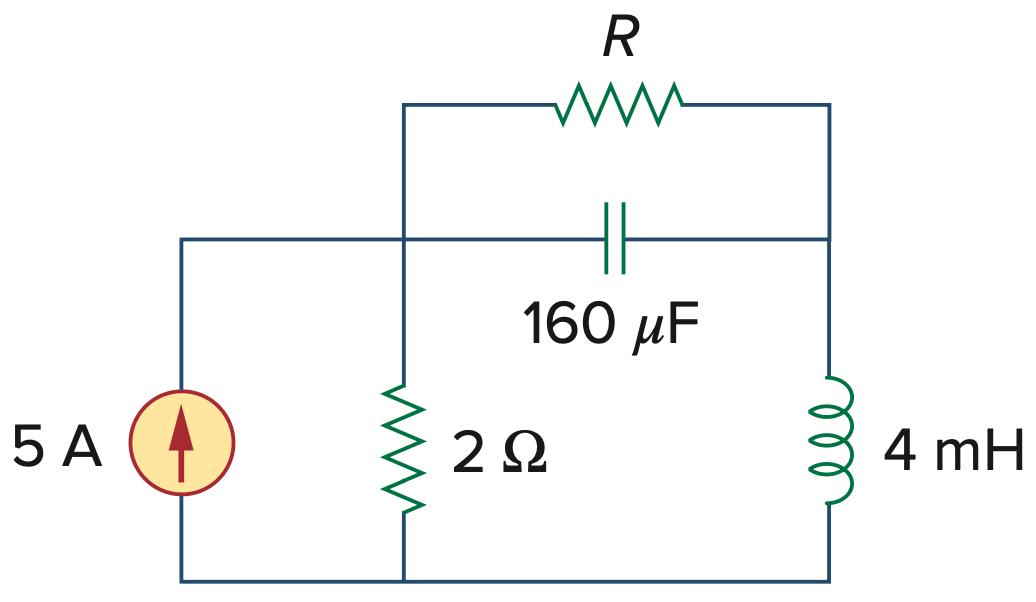
\includegraphics[width=0.7\textwidth]{figures/inductor_capacitor_circuit.png}
\end{exercise}

\ifshowsolutions
\begin{solution}
Bei stationärem Gleichstrom ist der Kondensator ein offener Stromkreis und die Induktivität ein Kurzschluss. Wir bezeichnen die Spannung am oberen Knoten mit $V$. Da der \(2\text{-}\Omega\)-Widerstand und $R$ beide mit Masse verbunden sind, gilt:
\[
\frac{V}{R} + \frac{V}{2\,\Omega} = 5\,\mathrm{A} \quad \Rightarrow \quad V = \frac{10R}{R+2}
\]

Der Gleichstrom durch die Induktivität entspricht dem Strom durch \(R\):
\[
I_L = \frac{V}{R} = \frac{10}{R + 2}
\]

Gleichsetzen der gespeicherten Energien:
\[
\frac{1}{2} C V^2 = \frac{1}{2} L I_L^2
\]

Ersetzen von \(V\) und \(I_L\) ergibt
\[
C \left( \frac{10 R}{R + 2} \right)^2 = L \left( \frac{10}{R + 2} \right)^2 \quad \Rightarrow \quad C R^2 = L,
\]

und somit

\[
R = \sqrt{\frac{L}{C}} = \sqrt{\frac{4 \times 10^{-3}}{160 \times 10^{-6}}}\,\Omega = 5\,\Omega.
\]
\end{solution}
\fi

% ----- Exercise 10 -----
\begin{exercise}[Serielle und Parallele Induktivitäten]
Bestimme $L_{\text{eq}}$ zwischen den Klemmen a-b von folgender Schaltung.

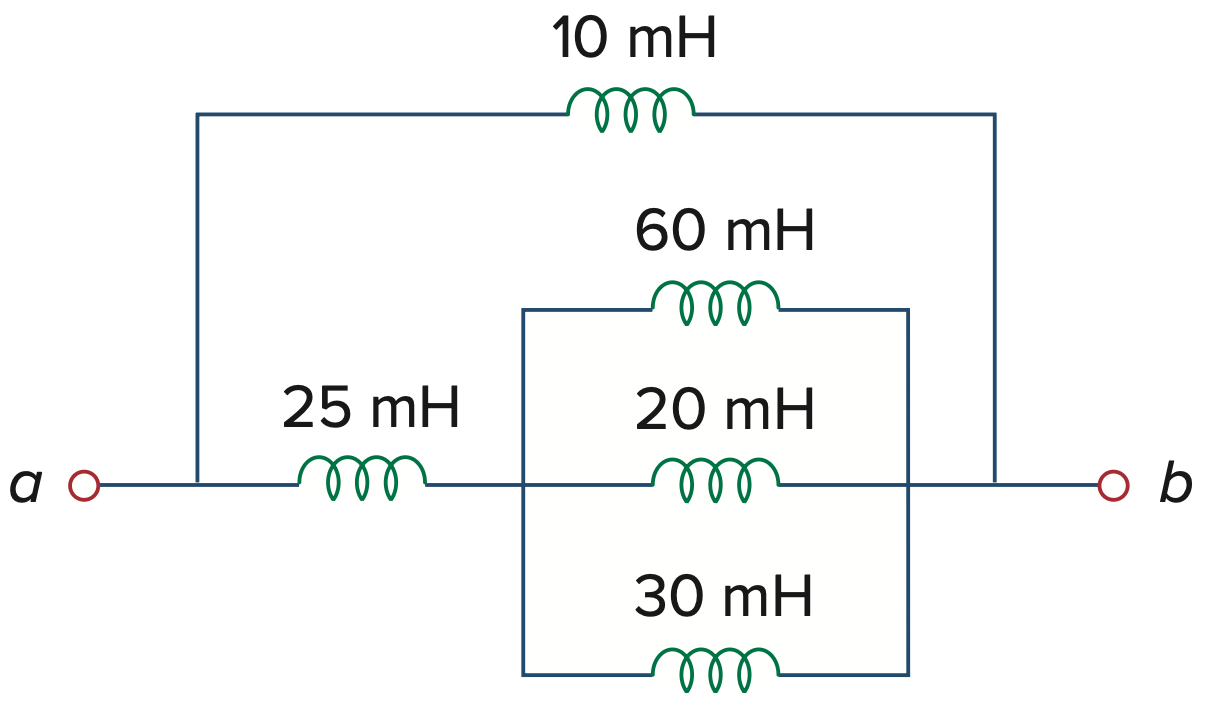
\includegraphics[width=0.7\textwidth]{figures/inductors_circuit.png}
\end{exercise}

\ifshowsolutions
\begin{solution}
Schritt 1: Parallelschaltung der drei Induktivitäten mit $60~\text{mH}$, $20~\text{mH}$, $30~\text{mH}$:
\[
\frac{1}{L_{\text{p}}} = \frac{1}{60~\text{mH}} + \frac{1}{20~\text{mH}} + \frac{1}{30~\text{mH}} = \frac{1}{10}~\frac{1}{\text{mH}}
\]
\[
\Rightarrow L_{\text{p}} = 10~\text{mH}
\]

Schritt 2: Reihenschaltung mit der Induktivität von $25~\text{mH}$:
\[
L_{\text{s}} = L_{\text{p}} + 25~\text{mH} = 10~\text{mH} + 25~\text{mH} = 35~\text{mH}
\]

Schritt 3: Parallelschaltung mit der Induktivität von $10~\text{mH}$:
\[
\frac{1}{L_{\text{eq}}} = \frac{1}{L_{\text{s}}} + \frac{1}{10~\text{mH}} = \frac{1}{35~\text{mH}} + \frac{1}{10~\text{mH}} = \frac{9}{70}~\frac{1}{\text{mH}}
\]
\[
\Rightarrow L_{\text{eq}} \approx 7.78~\text{mH}
\]
\end{solution}
\fi

\end{document}